%%%% Header %%%%%%%%%%%%%%%%%%%%%%%%%%%%%%%%%%%%%%%%%%%%%%%%%%%%%%%%%%%%%%%%%%%

\documentclass[12pt, parskip=half]{scrartcl}

\usepackage{jonas}

\bibliography{/home/jon/lucile/share/Dropbox/sci/refs/mendeley_bibtex/2016-09-imort_selection.bib}
\hyphenation{APGAR}

%%%% Meta data %%%%%%%%%%%%%%%%%%%%%%%%%%%%%%%%%%%%%%%%%%%%%%%%%%%%%%%%%%%%%%%%

\usepackage[
  pdfauthor   ={Jonas Schöley},
  pdftitle    ={Selection and adaptation components of infant mortality},
  %Decomposing the infant mortality age decline into direct and compositional effects
  pdfsubject  ={},
  pdfkeywords ={},
  pdfproducer =Latex,
  pdfcreator  =pdflatex
]{hyperref}

\title{Selection and adaptation components of infant mortality}
\author{
  Jonas Schöley\thanks{Max-Planck Odense Center on the Biodemography of Aging, University of Southern Denmark.}
  \and
  James Oeppen\footnotemark[1]
  \and
  Rune Lindahl-Jacobsen\footnotemark[1]
  \and
  James W.~Vaupel\thanks{Max Planck Institute for Demographic Research, Rostock, Germany.}~\footnotemark[1]
}

%%%% Titlepage %%%%%%%%%%%%%%%%%%%%%%%%%%%%%%%%%%%%%%%%%%%%%%%%%%%%%%%%%%%%%%%%

\begin{document}

\maketitle

\thispagestyle{empty}

\begin{abstract}
We test the selection hypothesis of infant mortality against the adaptation hypothesis by decomposing the mortality age pattern over the first year of life into an adaptation- and a selection component.  We show that the population level decline in mortality over the first hour of life is significantly influenced by mortality selection, i.e.~the frailest infants leaving the population shortly after birth. The subsequent mortality decline predominantly results from mortality changes observed in homogeneous sub-populations. This confirms the common view of the infant mortality age pattern being caused by adaptation on an individual level. The analysis is informed by detailed micro-data on births and infant deaths in the United States including more than 25 million births and 162,546 deaths. No parametric assumptions were necessary.
\end{abstract}

\clearpage

%%%% Text %%%%%%%%%%%%%%%%%%%%%%%%%%%%%%%%%%%%%%%%%%%%%%%%%%%%%%%%%%%%%%%%%%%%%

\section{Introduction}

% The phenomenon of ontogenescense
%For humans and many other species the hazard of death decreases from birth until onset of maturity (\cite{Medawar1952}). This phenomenon has been coined \enquote{ontogenescence} and various hypotheses have been suggested for its explanation (see \cite{Levitis2011} for an overview). The aim of this study is to examine these hypotheses using data on human fetal- and infant mortality, with the ultimate goal of explaining the phenomenon of ontogenescence for humans.


\section{Ontogenescence as growth and adaptation}

%The age pattern of infant mortality is commonly described as resulting from an \emph{adaptation process}. As the infant ages, it grows and acquires robustness, continuously increasing its resilience against death. The parametric mortality models by Siler (1979) and by Heligman and Pollard (1980) are examples of this line of thinking.\footnote{
%  \emph{\enquote{C measures the rate of mortality decline in childhood (the rate at which a child adapts to its environment)}} (\cite{Heligman1980}). \emph{\enquote{While the most common use of this decreasing hazard would be to account for the hazard due to immaturity, it can also be used [$\ldots$] for other hazards to which an animal adjusts successfully}} (\cite{Siler1979}).
%}

%1.~\emph{Individual level explanations:} The mortality decline over age observed on a population level is thought to originate from a declining hazard of death of each individual organism. Examples of individual level hypotheses are:
%  \emph{Growth-trade-off:} There is a trade-off between the current rate of growth and the current survival of an organism. Juvenile organisms who invest in fast growth momentarily worsen their survival chances with the prospect of increasing their adult survival once they have grown large (e.\,g.~\cite{Chu2008}).
%  \emph{Acquired Robustness:} As an individual growths in becomes more resilient towards death (e.\,g.~\cite{Munch2006}).
%  \emph{Transitional timing:} As the organism grows it has to pass a series of critical transitions, potentially dying at each. These transitions are concentrated early in life and therefore the mortality risk is concentrated in early life (\cite{Levitis2011}).

\section{Ontogenescence as mortality selection}

%An alternative explanation frames the declining force of mortality in early life as a \emph{selection process}. Infants who are born unfit for life will contribute heavily to the mortality rates observed right after birth. Due to this selection the mortality rate of the population will over time converge to the low-levels of the healthy survivors. These ideas can be formally expressed via the \enquote{frailty model}, a random effects proportional hazards model originally devised by \cite{Vaupel1979} in order to explain the old-age mortality deceleration. Various authors point to mortality selection as an explanation for the age pattern of infant mortality: \cite{Hougaard1984} points out that infant mortality can be modelled in a proportional hazards framework with a frailty factor $z$ coming from a distribution exhibiting extremely large variance and thereby capturing the inherent survival differences between infants born healthy and infants born with severe congenital disorders; \cite{Vaupel1985} show that two sub-populations with an age-constant hazard of differing magnitude will produce a declining hazard if grouped together; \cite{Levitis2011} explicitly names the \emph{heterogeneous frailty hypothesis} as a possible basis for the declining mortality before senescence. As of now however, the selection hypothesis remains untested.

%2.~\emph{Population level explanations:} The mortality decline over age is caused by mortality selection:\footnote{Within this article I relate the term \enquote{selection} solely to mortality without any implications for inheritance of specific traits as would be implied by its Darwinian meaning.} On average, the frailest individuals die first while the stronger individuals survive. Therefore, on the population level, the mean risk of death decreases over age. The \emph{Heterogeneous frailty} hypotheses (e.\,g.~\cite{Vaupel1985}) is an example for a population level hypothesis with a strong mathematical underpinning. A more specific example is \emph{Quality control:} the frailest die first, terminated by their kin (\cite{Hamilton1966}).

%Prior work on selection in fetal- and infant mortality was conducted in the context of the \emph{fetal origins hypothesis} \autocite{Barker1990}, or more generally, \emph{late life legacies of early life conditions} \autocite{Doblhammer2003}, in research on \emph{fetal culling} \autocite{Catalano2006}, and in applications and developments of the \emph{frailty model}. The latter excluded, these research programmes concern the health and mortality consequences of risk-exposure early in life. Two competing mechanisms have been identified: \emph{scarring} and \emph{selection}. A cohort is scarred when the survival prospects of its members are lowered following an exposure to risk. Selection takes place if the cohorts' survival prospects are increased following the exposure (due to the survival of the healthiest). While both processes might act simultaneously, studies tend to focus on one or the other mechanism.

%\textcite{Piccione2014} find an inverse relationship between mortality levels during the first 3 months of life and the subsequent 32 months. \enquote{No Increased Mortality in Later Life for Cohorts Born during Famine} has been found by \autocite{Kannisto1997}. The authors note that \enquote{selection bias} might have confounded the results, with a famine selecting for the healthiest members of a population. \textcite{Doblhammer2001} find that \enquote{Lifespan depends on month of birth}. The authors recognize \enquote{selective survival in the first year of life} as a possible explanation for this result but refute it in favour of the \enquote{debilitation in utero or in infancy} hypothesis \autocite[p.~2938]{Doblhammer2001}. Noting that the impact of social class on the risk of fetal death decreases during the third trimester of a pregnancy, \autocite{Carlson1999} argue (but don't test) that selection leads to a homogenisation of the fetal population in terms of risk-factors. A series of papers on the \enquote{culled cohorts} hypothesis presents indirect evidence for intrauterine mortality selection changing the composition of a cohort in terms of health and survival \autocite{Catalano2006, Bruckner2007, Bruckner2013}.

%The process of mortality selection has been formalized into the \emph{frailty model}. Originally specified as a random effects proportional hazards model using life table notation \autocite{Vaupel1979} the model has been extended and thoroughly discussed and explored over time \autocite[][e.g.]{Wienke2011, Duchateau2008, Vaupel2014}. While it has mostly been used to explain the old-age mortality plateau in terms of selection, various authors point out the possibilities to model infant mortality using a frailty model: \textcite{Hougaard1984} briefly remarks that infant mortality can be modelled in a proportional hazards framework with a frailty factor $z$ coming from a distribution exhibiting extremely large variance and thereby capturing the inherent survival differences between infants born healthy and infants born with severe congenital disorders; \textcite{Vaupel1985} show that two sub-populations with an age-constant hazard of differing magnitude will produce a declining hazard if grouped together; \textcite{Levitis2011} explicitly names the \emph{heterogeneous frailty hypothesis} as a possible basis for the declining mortality before senescence. While being proposed numerous times I can find only a single instance where a frailty model has actually been fitted to infant mortality data. \textcite{Feaganes1993} incorporates frailty into Weibull- and Poisson regression models on infant mortality in order to estimate coefficients unbiased by unobserved heterogeneity. \textcite{Berrut2016a} -- without referring to frailty models -- recognize the difference between individual level changes in infant mortality over age and population level selection effects and argue that birth constitutes a transitional shock selecting those out of the population who are unfit for life.\footnote{This publication is quite remarkable inasmuch it is published in a physics journal and the authors are largely ignorant on demographic-, medical- or epidemiological work on the age-pattern of fetal- and infant mortality.}

%\emph{While selection in fetal- and infant mortality is \emph{discussed} in the literature it hasn't been systematically \emph{studied} in its own right with regard to the age-pattern of mortality.}

\section{Decomposition methods}

Consider a cohort of newborns stratified into sub-populations $i=1\ldots k$ according to mortality relevant characteristics (e.\,g.~birth-weight, gestation at birth, presence of congenital diseases etc.). For each time-point during infancy we estimate the hazard of death for both the total population ($\overbar{\mu}(x)$)and each sub population ($\mu_i(x)$) as well as the composition of survivors $p_i(x)$. Given time points $x_2 > x_1$, how much of the difference of the population hazard at these points is explained by a change of the sub-population hazards and how much due to a change in the population composition?

Decomposition problems similar to the one stated above have been tackled by many fields over the last half century. The proposed solutions can be categorized as either parametric and regression based (e.g. Oaxaca, Blinder, Powers) or non-parametric and co-variance based (e.g. Price, Preston, Vaupel-Canadas-Romo, Rebke). The latter approach has been formulated using life-table notation, uses aggregate level data and will be quite intuitive to demographers. The regression based approach on the other hand allows for the direct use of individual level survival data which facilitates multivariate decompositions (while multivariate extensions of co-variance based approaches exist, they require the calculation of a life-table for each observed combination of variable levels, which, while far from infeasible, is rather inconvenient. Furthermore continuous variables have to be discretized which is not the case for the regression based decompositions).

We will demonstrate two different decomposition approaches: a non-parametric, univariate composition proposed by \autocite{Vaupel2002} and a multivariate, Poisson-regression based decomposition by \autocite{Powers2011}. Vaupel etals.~method requires aggregate level life-table data and is stated in standard demographic notation. It therefore serves as an intuitive introduction to the decomposition problem. Powers' method -- a regression based extension of the asdf decomposition -- requires individual level survival data and allows to assess the relative contribution of multiple co-variates to the overall selection effect.



%The methodological foundation for this decomposition goes back to the \emph{Price equation}, a fundamental theorem in evolutionary biology stating how traits in a population change both due to changes in traits between parents and offspring and due to natural selection of traits leading to higher fitness. It has been noted that this relation can also be applied to mortality schedules in a population \autocite{Rebke2012}.\footnote{
%  Without being aware of its original use in evolutionary biology demographers have used expressions similar to the Price equation in decomposition analysis \autocite[see][]{Preston2011a, Schoen1992, Vaupel2002}.
%} Substituting \enquote{trait} by \enquote{mortality level} and \enquote{parents/offspring} by \enquote{age $x$ and $x+1$} yields a decomposition method for individual and population level changes in age patterns of mortality. \textcite{Vaupel2010a} express this relationship as:

%\begin{equation}
%  \dot{\overline{\mu}}(x) = \overline{\dot{\mu}}(x) - \sigma^2_\mu(x),
%  \label{eq:dec}
%\end{equation}

%the momentary change in average mortality at age $x$ equals the average change in mortality minus the variance of mortalities at the same age.\footnote{
%  Although formulated in continuous fashion this relationship extends to the discrete setting as well.
%} All terms in this equation can be calculated from a collection of life tables stratified over groups of a cohort. A generalization of the Price equation \autocite{Kerr2009} allows decomposition into multiple selection components (this is important in the fetal case where natural death, induced abortion and birth all have a selective effect on the population).

\section{Data}

%We use publicly available microdata on fetal deaths, live births and infant deaths in the United States provided by the National Center for Health Statistics.

%The \enquote{birth cohort linked birth-infant death data files} \autocite{NCHS2016} contain information on all children born 1983--91 and 1995--2010 in the United States (U.S.) and -- as a subset of this population -- all infant deaths (deaths occurring prior to the first birthday of a child) occurring in the U.S.~related to these birth cohorts. Individual birth- and death certificates form the basis for the information given in the data set. These certificates ensure harmonized reporting across the states and each contain more than 50 items containing demographic information on child, father and mother, medical status of the newborn, complications of pregnancy and labour, risk factors during the pregnancy, procedures during pregnancy and labour, time of death and cause of death. No data was published for the years 1992--1994 \autocite{Weed1995}.

%The \enquote{fetal death data files} \autocite{NCHS2016a} cover fetal deaths occurring 1982-2013 in the U.S. In accordance with the WHO definition of fetal death, induced abortions are \emph{not} part of the data \autocite{Kowaleski1997}. While reporting standards vary between states all but three states report fetal deaths at 20 weeks of gestation or more \autocite{Kowaleski1997}.\footnote{New Mexico, South Dakota, and Tennessee require a weight at delivery of 500 grams or more for a fetal death report to be filled.}

%For fetal death data including induced abortions and earlier periods of gestation I will apply for access to the \enquote{Medical Birth Registry of Norway}\footnote{
%  Despite its name this database tracks pregnancies as well as births.
%} \autocite{Irgens2000} and to Danish register data.

%\emph{The available data allow us to calculate age-specific death rates for fetal- and infant death and capture an immense amount of heterogeneity in these rates via stratification by covariates, thereby allowing decomposition of the age-pattern of mortality in adaptation- and selection effects.}

\section{Univariate decomposition}

\begin{figure}[!htb]
  \centering
  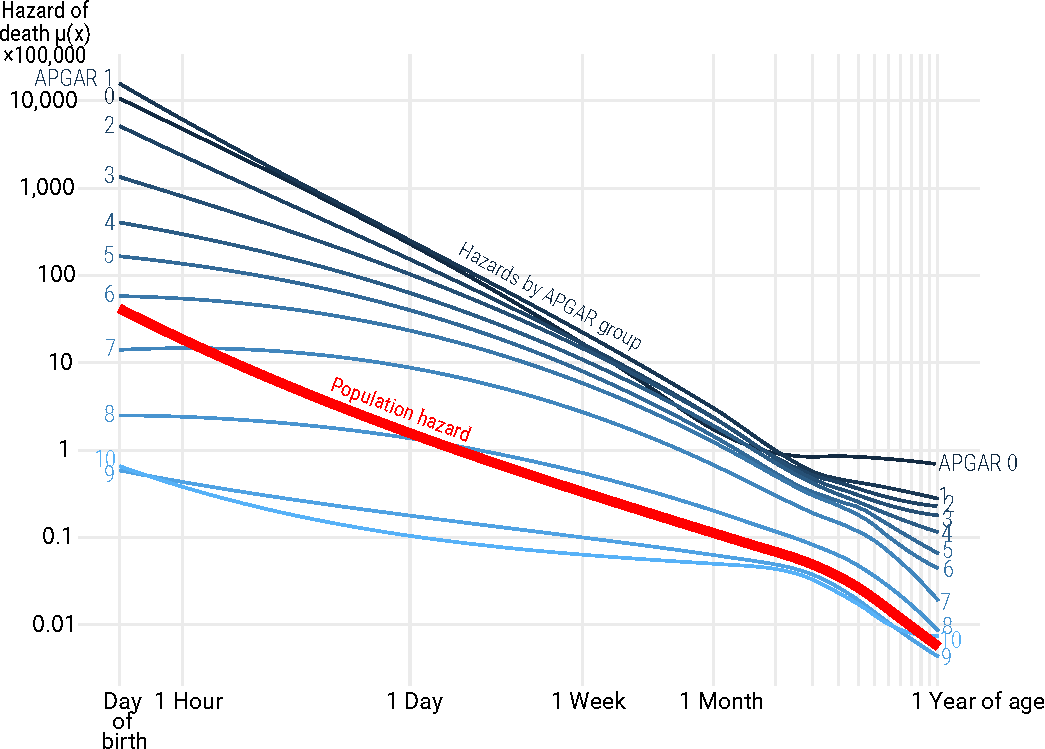
\includegraphics[width = .9\textwidth]{./fig/plot_ilt_dob0510_apgar5.pdf}
  \caption{\textsc{Hazard of death over the first year of life for infants born in the US 2005--10 by 5 minute APGAR score and on aggregate.} All APGAR groups experience some degree of mortality decline though the shape and speed of that decline varies. The effect of mortality selection can clearly be seen by the population hazard approaching the hazard of the high-APGAR groups (e.g. those with a survival advantage). The hourly/daily mortality rates have been LOESS-smoothed prior to plotting. Data: Calculated on the basis of the birth cohort linked birth-infant death data files by the National Center for Health Statistics.}
  \label{fig:apgar}
\end{figure}

%In the first analysis presented here I use the \emph{APGAR} score, one of the best predictors for the risk of infant death, as the variable stratifying the population into homogeneous groups. The APGAR score measures the overall vitality of a newborn on a scale from 0 (no vital signs) to 10 (strongest vital signs) and can be regarded as a very good proxy for the (inverse-) frailty of a child. Using publicly available microdata on live births and infant deaths in the United States provided by the National Center for Health Statistics I calculate life-tables over day of age for each of the APGAR scores.

Figure \ref{fig:apgar} shows the hazard of death (smoothed from hourly/daily mortality rates). As expected the general level of mortality is ordered by the APGAR score with higher scores associated with lower mortality. All groups experience some degree of mortality decline though the shape and speed of that decline varies. The effect of mortality selection can clearly be seen by the population hazard approaching the hazard of the high-APGAR groups (e.g.~those with a survival advantage).

%Using equation \ref{eq:dec} I decompose the age-to-age-change in the population hazard and find that mortality selection causes 21.8\,\% of the aggregate mortality decline between the first hour of life and the end of the first day of life. For subsequent ages the mortality selection plays no significant role in shaping the aggregate age pattern (see table \ref{tab:decomp}).

\begin{table}[!htb]
  \tabformat
  \begin{threeparttable}
    \begin{tabular}{p{2.5cm}p{2cm}p{2cm}p{2.7cm}}
      \toprule
      Age interval of mortality change & Adaptation component $\bar{\dot{\mu}}(x)$ & Selection component $-\sigma^2_\mu(x)$ & \%\,of mortality change attributable to selection \\
      \midrule
      First hour of life & -6.32e-02 & -1.76e-02 & 21.8 \\
      Hours 1--24        & -4.24e-03 & -7.50e-05 &  1.7 \\
      Day 1              & -2.28e-04 & -4.53e-07 &  0.2 \\
      Day 2              & -1.08e-04 & -1.04e-07 &  0.0 \\
      Day 3              & -5.88e-05 & -5.10e-08 &  0.0 \\
      Day 4              & -3.33e-05 & -2.59e-08 &  0.0 \\
      Day 5              & -1.75e-05 & -1.29e-08 &  0.0 \\
      \bottomrule
    \end{tabular}
    \begin{tablenotes} \tabfontsizefoot
      \item Data: Calculated on the basis of the birth cohort linked birth-infant death data files by the National Center for Health Statistics.
    \end{tablenotes}
    \caption{Decomposition of the change in the population hazard into adaptation and selection components for infants born in the US 2005--10: 21.8\,\% of the decline in the population mortality hazard between the first hour of life and the remainder of the first day of life are explained by mortality selection due to heterogeneity between sub-groups with different APGAR score.}
    \label{tab:decomp}
  \end{threeparttable}
\end{table}

\section{Multivariate decomposition}

\begin{table}[!htb]
  \tabformat
  \begin{threeparttable}
    \begin{tabular}{ll*{2}{p{1cm}}*{5}{p{1cm}}}
      \toprule
       & & \multicolumn{2}{c}{$\Delta\mu(x)$ due to} & \multicolumn{5}{c}{Share on compositional change} \\
      \cmidrule(r){3-4}\cmidrule(l){5-9}
      Age interval & Total $\Delta\mu(x)$ & direct change & compos. change & sex & birth-weight & birth defect & 5 min APGAR & Mother's social status \\
      \midrule
      Hour 0 to 24 & 2.86E-03 & 39.4 & 60.6 & 0.00 & 0.16 & 0.04 & 0.80 & 0.00 \\
      Day 2 to 7 & 7.84E-06 & 85.5 & 14.5 & 0.00 & 0.27 & 0.13 & 0.59 & 0.01 \\
      Week 2 to 4 & 1.72E-06 & 91.7 & 8.3 & 0.00 & 0.25 & 0.24 & 0.49 & 0.02 \\
      Month 2 to 12 & 1.69E-06 & 93.7 & 6.3 & 0.00 & 0.52 & 0.20 & 0.28 & 0.00 \\
      \bottomrule
    \end{tabular}
    \begin{tablenotes} \tabfontsizefoot
      \item Data: Calculated on the basis of the birth cohort linked birth-infant death data files by the National Center for Health Statistics.
    \end{tablenotes}
    \caption{Decomposition of the change in the population hazard into adaptation and selection components for infants born in the US 2005--10: 60.6\,\% of the decline in the population mortality hazard over the first day of life are explained by mortality selection. The differences in APGAR score explain 80\,\% of the total selection effect.}
    \label{tab:decomp}
  \end{threeparttable}
\end{table}

\section{Discussion}

Mortality selection drives the mortality decline immediately after birth. Still, most of the infant mortality decline over age is due to individual level effects, i.\,e.~a growing resilience of the individual as it ages.

\clearpage

%%%% Bibliography %%%%%%%%%%%%%%%%%%%%%%%%%%%%%%%%%%%%%%%%%%%%%%%%%%%%%%%%%%%%%

\sloppy
\printbibliography

%\clearpage

%%%% Appendix %%%%%%%%%%%%%%%%%%%%%%%%%%%%%%%%%%%%%%%%%%%%%%%%%%%%%%%%%%%%%%%%%

% appendix figures follow A1, A2, B1... scheme
%\renewcommand\thefigure{\thesection.\arabic{figure}}
%\setcounter{figure}{0}

\end{document}